%% ****** Start of file apstemplate.tex ****** %
%%
%%
%%   This file is part of the APS files in the REVTeX 4.2 distribution.
%%   Version 4.2a of REVTeX, January, 2015
%%
%%
%%   Copyright (c) 2015 The American Physical Society.
%%
%%   See the REVTeX 4 README file for restrictions and more information.
%%
%
% This is a template for producing manuscripts for use with REVTEX 4.2
% Copy this file to another name and then work on that file.
% That way, you always have this original template file to use.
%
% Group addresses by affiliation; use superscriptaddress for long
% author lists, or if there are many overlapping affiliations.
% For Phys. Rev. appearance, change preprint to twocolumn.
% Choose pra, prb, prc, prd, pre, prl, prstab, prstper, or rmp for journal
%  Add 'draft' option to mark overfull boxes with black boxes
%  Add 'showkeys' option to make keywords appear
\documentclass[aps,prl,twocolumn,groupedaddress]{revtex4-2}
%\documentclass[aps,prl,preprint,superscriptaddress]{revtex4-2}
%\documentclass[aps,prl,reprint,groupedaddress]{revtex4-2}
\usepackage{natbib}
\usepackage[export]{adjustbox}
\usepackage{graphicx}
\usepackage{float}
\usepackage{braket}
\usepackage[utf8]{inputenc}
\usepackage[utf8]{ctex}

% You should use BibTeX and apsrev.bst for references
% Choosing a journal automatically selects the correct APS
% BibTeX style file (bst file), so only uncomment the line
% below if necessary.
%\bibliographystyle{apsrev4-2}

\begin{document}

% Use the \preprint command to place your local institutional report
% number in the upper righthand corner of the title page in preprint mode.
% Multiple \preprint commands are allowed.
% Use the 'preprintnumbers' class option to override journal defaults
% to display numbers if necessary
%\preprint{}

%Title of paper
\title{二维零场 Ising 模型的 Monte Carlo 数值模拟}

% repeat the \author .. \affiliation  etc. as needed
% \email, \thanks, \homepage, \altaffiliation all apply to the current
% author. Explanatory text should go in the []'s, actual e-mail
% address or url should go in the {}'s for \email and \homepage.
% Please use the appropriate macro foreach each type of information

% \affiliation command applies to all authors since the last
% \affiliation command. The \affiliation command should follow the
% other information
% \affiliation can be followed by \email, \homepage, \thanks as well.
\author{林照翔}
%\email[]{Your e-mail address}
%\homepage[]{Your web page}
%\thanks{}
%\altaffiliation{}
\affiliation{兰州大学物理科学与技术学院2022理论2班}

%Collaboration name if desired (requires use of superscriptaddress
%option in \documentclass). \noaffiliation is required (may also be
%used with the \author command).
%\collaboration can be followed by \email, \homepage, \thanks as well.
%\collaboration{}
%\noaffiliation

\date{\today}

\begin{abstract}
% insert abstract here
本文使用 Single-spin-flip Dynamics 方法和 Cluster-flip Dynamics 方法\cite{01}对二维零场 Ising 模型进行数值模拟。
\end{abstract}

% insert suggested keywords - APS authors don't need to do this
% \keywords{}

%\maketitle must follow title, authors, abstract, and keywords
\maketitle

% body of paper here - Use proper section commands
% References should be done using the \cite, \ref, and \label commands
\section{I. 引言}

% Put \label in argument of \section for cross-referencing
%\section{\label{}}
伊辛模型\cite{03}的提出是为了解释铁磁物质的相变,即磁铁在加热到一定临界温度以上会出现磁性消失的现象,而降温到临界温度以下又会表现出磁性。这种有磁性、无磁性两相之间的转变,是一种连续相变(也叫二级相变)。伊辛模型假设铁磁物质是由一堆规则排列的小磁针构成,每个磁针只有上下两个方向(自旋)。相邻的小磁针之间通过能量约束发生相互作用,同时又会由于环境热噪声的干扰而发生磁性的随机转变(上变为下或反之)。涨落的大小由关键的温度参数决定,温度越高,随机涨落干扰越强,小磁针越容易发生无序而剧烈地状态转变,从而让上下两个方向的磁性相互抵消,整个系统消失磁性,如果温度很低,则小磁针相对宁静,系统处于能量约束高的状态,大量的小磁针方向一致,铁磁系统展现出磁性。

\section{II. 二维零场 Ising 模型}

\subsection{A. 二维零场 Ising 模型哈密顿量}

考虑二维晶格,每个格点的自旋 $\sigma_i $ 要么向上,要么向下,即:

$$
\sigma_i \in \left\{1,-1 \right\}
$$

两个相邻的自旋 $i,j $ 之间存在自旋交互作用,每个自旋与磁场也存在交互作用。引入交互作用常量 $J_{ij} $,将并格点 $j $ 上的磁场记为 $h_j $,则整个系统的哈密顿量 $H $ 可写为:

$$
H(\sigma)
=-\sum_{\braket{i,j}} J_{ij} \sigma_i \sigma_j - \mu \sum_{j} h_j \sigma_j
$$

其中,$\sigma\equiv \left\{\sigma_1,\sigma_2,\cdots,\sigma_N \right\} $ 是 $N $ 个自旋的取向,称为位形;$\braket{i,j} $ 表示对最近邻的格点求和(每一对只计算一次);$\mu $ 代表磁矩。

考虑外加磁场为零,且所有相邻自旋的交互作用都是相等的的情况,即:

$$
h_j = 0,\quad 
J_{ij} = J
$$

此时,系统的哈密顿量可简化为:

$$
H
=-J \sum_{\braket{i,j}} \sigma_i\sigma_j
$$

\subsection{B. 重要性抽样}

一般的宏观系统中,$N\sim 10^{23} $,系统共有 $2^N\sim 2^{10^{23}} $ 种位形,遍历所有位形计算哈密顿量的是不可能的。

为了避免遍历所有位形带来的海量计算,可以采用 Monte Carlo 算法,即从整体中以一定方式抽取样本,通过计算样本的统计学量来估计整体的统计学量。

根据样本的重要性来决定抽样密度的方法称为重要性抽样。

以玻尔兹曼系统为例,热力学量 $Q $ 的平均值 $\braket{Q} $ 的定义为系综平均值,即:

$$
\braket{Q}
\equiv \frac{\sum\limits_{\sigma} Q(\sigma) \mathrm{e}^{-\beta H(\sigma)} }{\sum\limits_{\sigma} \mathrm{e}^{-\beta H(\sigma)}} 
$$

在玻尔兹曼系统中,位形 $\sigma $ 出现的概率正比于 $\mathrm{e}^{-\beta H(\sigma)} $,因此合理的抽样方式应是对位形 $\sigma $ 以 $P(\sigma)\propto \mathrm{e}^{-\beta H(\sigma)} $ 进行重要性抽样。

假设通过上述重要性抽样共抽取了 $M $ 个样本位形 $\tilde{\sigma}_1,\tilde{\sigma}_2,\cdots,\tilde{\sigma}_M $ ,则可取这 $M $ 个样本中热力学量 $Q $ 的统计平均值作为对其系综平均的近似,即:

$$
\braket{Q}
\approx \frac{\sum\limits_{i=1}^{M} Q\left(\tilde{\sigma}_i \right) }{M } 
$$

\section{III. 马尔可夫过程}

\subsection{A. 马尔可夫过程(马尔可夫链)}

马尔可夫过程是一个具备了马尔可夫性质的随机过程,因为俄国数学家安德雷·马尔可夫得名。马尔可夫过程是不具备记忆特质的。换言之,马尔可夫过程的条件概率仅仅与系统的当前状态相关,而与它的过去历史或未来状态,都是独立、不相关的。

马尔可夫链是满足马尔可夫性质的随机变量序列 $X_1, X_2, X_3,\cdots $,某一个状态 $X_{n+1} $ 仅与前一个状态 $X_n $ 有关,即:

$$
\mathrm{P}\left(X_{n+1} = x | X_1=x_1,\cdots,X_n=x_n \right)
=\mathrm{P}\left(X_{n+1}=x | X_n = x_n \right)
$$

\subsection{B. “好”马尔可夫过程的稳态分布}

我们用 $P_{\mu\to \nu} $ 表示系统从状态 $\mu $ 转移到状态 $\nu $ 的概率。

对于一个“好”马尔可夫过程,无论初始状态是什么,只要经历足够多的步数,末态的概率分布是确定的,这个末状态称为稳态。

我们用稳态概率分布(简称稳态分布) $P(\mu) $ 来表示稳态时系统处于状态 $\mu $ 的概率。

\subsection{C. “好”马尔可夫过程需要满足的条件}

一个“好”马尔可夫过程要满足以下两个条件:

(1)遍历性:无论从哪个状态出发,都能找到一条概率不为零的路径达到任意状态。

(2)细致平衡:稳态概率分布和转移概率满足:

$$
P(\mu)P_{\mu\to \nu} = P(\nu) P_{\nu\to \mu}
$$

我们可以选定一个选择概率 $g(\mu,\nu) $,表示当系统处于状态 $\mu $ 时,在所有可能的状态中选择状态 $j $ 的概率。

另外还需要定义一个接受概率 $A(\mu,\nu) $,表示当系统处于状态 $\mu $ 时,接受系统跳转到状态 $\nu $ 的概率。

可以看到,$g(\mu,\nu)A(\mu,\nu) $ 就是马尔可夫过程中的转移概率 $P_{\mu\to \nu} $,即:

$$
P_{\mu\to \nu} = g(\mu,\nu)A(\mu,\nu)
$$

因此,细致平衡条件也可以通过选择概率和接受概率表达为:

$$
P(\mu)g(\mu,\nu)A(\mu,\nu) = P(\nu)g(\nu,\mu)A(\nu,\mu)
$$

\section{IV. Ising 模型的 Monte Carlo 解}

回到二维零场 Ising 模型,我们希望对位形 $\sigma $ 以概率 $P(\sigma)\propto \mathrm{e}^{-\beta H(\sigma)} $ 进行重要性抽样。这可以通过“好”的马尔可夫过程实现。

我们可以构造一个特殊的“好”马尔可夫过程,使得其稳态关于位形 $\sigma $ 的稳态分布 $P(\sigma) $ 满足 $P(\sigma)\propto \mathrm{e}^{-\beta H(\sigma)} $,这样就能实现对位形 $\sigma $ 以概率 $P(\sigma)\propto \mathrm{e}^{-\beta H(\sigma)} $ 进行重要性抽样。

\subsection{A. Single-spin-flip Dynamics 方法}

Single-Spin-Flip-Dynamics 是一个“好”的马尔可夫过程。在热平衡时,整个 Ising 系统的能量只会有小幅度的扰动,这点促成了在演算时采用单一自旋反转法进行计算,也就是说每次系统跳转其位形时,只改变其中一个自旋的方向。

由于我们一次只翻转一个自旋,即位形跳转前后的位形仅有一个方向不同的自旋。因此,当位形 $\mu $ 和位形 $\nu $ 不满足“仅有一个方向不同的自旋”这一条件时,我们拒绝从位形 $\mu $ 跳转到位形 $\nu $,即:

$$
P_{\mu\to \nu}= 0
$$

下面考虑位形 $\mu $ 和 位形 $\nu $ 仅有一个方向不同的自旋的情况。

为简单起见,对于任何一个状态 $\mu $,认为它以相同概率选择 $N $ 个格点中的一个进行自旋翻转,即人为规定选择几率满足:

$$
g(\mu,\nu) = 1/N
$$

为实现重要性抽样,我们希望稳态分布满足 $P(\mu)\propto \mathrm{e}^{-\beta H(\mu)},P(\nu)\propto \mathrm{e}^{-\beta H(\nu)} $,因此有:

$$
\frac{P(\mu) }{P(\nu) } 
=\frac{\mathrm{e}^{-\beta H(\mu)} }{\mathrm{e}^{-\beta H(\nu)} } 
=\mathrm{e}^{-\beta \left[H(\mu)-H(\nu) \right]}
$$

将稳态分布条件和选择概率代入细致平衡条件,得到接受概率应满足的条件:

$$
\frac{A(\mu,\nu) }{A(\nu,\mu) } = \mathrm{e}^{-\beta \left[H(\nu)-H(\mu) \right]}
$$

满足上式的接受概率的一种可能取法是 Metropolis 接受准则,即如下的接受概率:

$$
A(\mu,\nu)
=\left\{
\begin{array}{ll}
\mathrm{e}^{-\beta\left[H(\nu)-H(\mu) \right]}&,\quad H(\nu)-H(\mu)>0 \\
1 &,\quad \mathrm{otherwise.}
\end{array}
\right.
$$

注意到,位形 $\nu $ 与 位形$\mu $ 仅有一个方向不同的自旋。设位形 $\mu$ 把自旋 $\sigma_k$ 翻转为 $-\sigma_k$ 从而跳转到位形 $\nu$,设 $\sigma_k $ 的四个最近邻自旋分别为 $\sigma_{k1},\sigma_{k2},\sigma_{k3},\sigma_{k4} $,则跳转前后的能量差为:

$$
H(\nu)-H(\mu)
=2J\sigma_k(\sigma_{k1}+\sigma_{k2}+\sigma_{k3}+\sigma_{k1})
$$

Single-Spin-Flip-Dynamics 方法稳态时重要性抽样的具体步骤如下:

(1)以 $1/N $ 的选择概率选出一个自旋,并计算自旋翻转前后能量差 $H(\nu)-H(\mu) $;

(2)如果能量差 $H(\nu)-H(\mu)\leq 0 $,翻转选择的自旋;

(3)如果能量差 $H(\nu)-H(\mu)> 0 $,则以 $ \mathrm{e}^{-\beta\left(H_j-H_i \right)} $ 的概率翻转选择的自旋;

(4)记录当前位形下热力学量的取值;

(5)重复步骤(1)。

\begin{figure}[htbp]
    \centering
    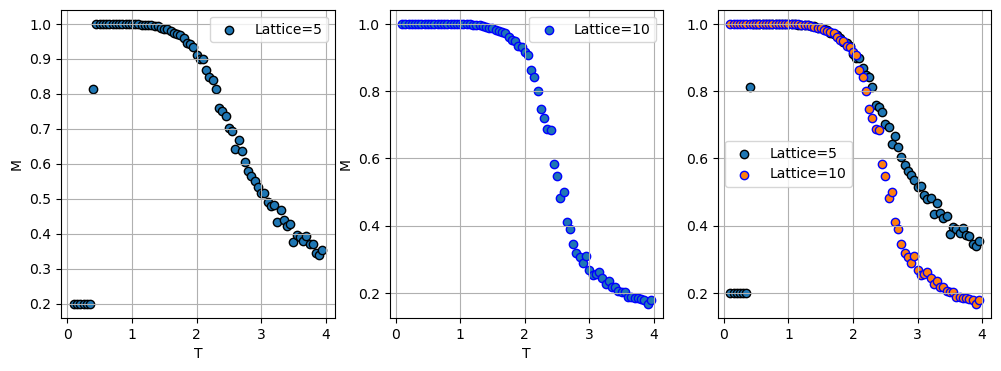
\includegraphics[width=0.55\textwidth]{img/fig1.png}
    \caption{平均磁矩随温度变化关系(取 $k=J=1$)理论\cite{02}给出在 $T_c=2/\ln(1+\sqrt{2})\approx 2.269 $ 处 发生相变}
    \label{fig1}
\end{figure}

\begin{figure}[htbp]
    \centering
    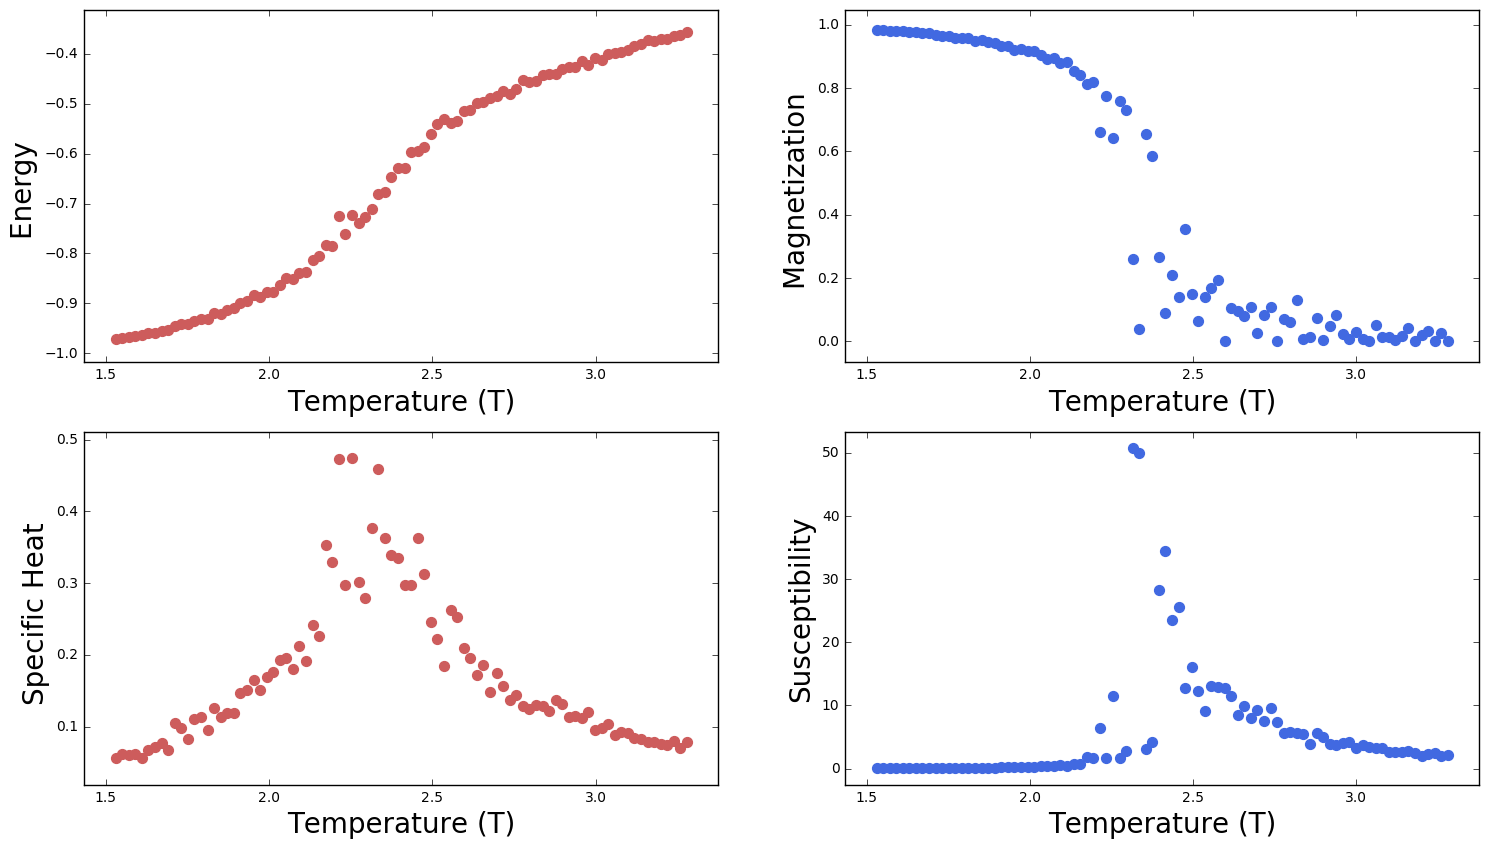
\includegraphics[width=0.55\textwidth]{img/fig2.png}
    \caption{其他热力学量随温度变化关系(取 $k=J=1$)}
    \label{fig2}
\end{figure}

\subsection{B. Cluster-flip Dynamics 方法}

与 Single-Spin-Flip-Dynamics 方法单步翻转单个自旋不同,Cluster-flip-Dynamics 方法单步会翻转多个自旋。每次被翻转的自旋簇称为 cluster.

Cluster-flip-Dynamics 方法稳态时重要性抽样的具体步骤如下:

(1)在系统中随机抽取一个自旋作为种子;

(2)以 $\mathrm{P}_{\mathrm{add}} $ 的概率依次决定是否添加种子周围的同向自旋到 cluster中;

(3)把原来的种子标记为 operated,把新加入的自旋作为新的种子;

(4)重复步骤(2)(3),直到 cluster 中所有的自旋都被标记为 operated,即不再有新的种子;

(5)以 $A_{\mu,\nu} $ 的概率翻转 cluster;

(6)记录当前位形下热力学量的取值;

(7)重复步骤(1)。

\subsubsection{1. $\text{Wolff}$ 算法}

这里,我们仍需要构造“好”的马尔可夫过程,因此仍要满足细致平衡条件。

当前系统的位形记为 $\mu $,设 cluster-flip 把位形 $\mu $ 中一个自旋为 $\sigma $ 的 cluster 全部翻转为 $-\sigma $ 从而跳转到位形 $\nu $,设最近邻包围被翻转的 cluster 的所有自旋中自旋为 $\sigma $ 的有 $m $ 个,自旋为 $-\sigma $ 的有 $n $ 个,则系统处于位形 $\mu $ 时选择位形 $\nu $ 的选择概率 $g(\mu,\nu) $ 可以人为规定为:

$$
g(\mu,\nu) = \left(1-\mathrm{P}_{\mathrm{add}} \right)^m
$$

容易得到:

$$
g(\nu,\mu) = \left(1-\mathrm{P}_{\mathrm{add}} \right)^n
$$

因此:

$$
\frac{g(\mu,\nu) }{g(\nu,\mu) } = \frac{\left(1-\mathrm{P}_{\mathrm{add}} \right)^m }{\left(1-\mathrm{P}_{\mathrm{add}} \right)^n} 
=\left(1-\mathrm{P}_{\mathrm{add}} \right)^{m-n}
$$

细致平衡条件:

$$
P(\mu) g(\mu,\nu) A(\mu,\nu) = P(\nu) g(\nu,\mu) A(\nu,\mu)
$$

我们希望稳态分布满足:

$$
P(\mu) \propto \mathrm{e}^{-\beta H(\mu)},\quad 
P(\nu) \propto \mathrm{e}^{-\beta H(\nu)}
$$

因此:

$$
\frac{P(\mu) }{P(\nu) } = \mathrm{e}^{-\beta \left[H(\mu)-H(\nu) \right]}
$$

把概率密度分布和选择概率代入细致平衡条件,可得:

$$
\frac{A(\mu,\nu) }{A(\nu,\mu) } 
=\frac{P(\nu) }{P(\mu) } \frac{g(\nu,\mu) }{g(\mu,\nu) } 
=\mathrm{e}^{-\beta\left[H(\nu)-H(\mu) \right]} \left(1-\mathrm{P_{add}} \right)^{n-m}
$$

注意到:

$$
H(\nu)-H(\mu) = 2(m-n)J
$$

因此,接受概率要满足:

$$
\frac{A(\mu,\nu) }{A(\nu,\mu) } 
=\mathrm{e}^{-2\beta (m-n)J}\left(1-\mathrm{P_{add}} \right)^{n-m}
$$

特别地,若把 $\mathrm{P}_{\mathrm{add}} $ 取为:

$$
\mathrm{P_{add}}
=1-\mathrm{e}^{-2\beta J}
$$

则接受概率要满足:

$$
\frac{A(\mu,\nu) }{A(\nu,\mu) } 
=\mathrm{e}^{-2\beta (m-n)J}\cdot \mathrm{e}^{-2\beta J(n-m)}
=1
$$

因此,一种简单的接受概率取法就是:

$$
A(\mu,\nu)
=1
$$

即只要构造出了 cluster 就对其进行翻转。

\begin{figure}[htbp]
    \centering
    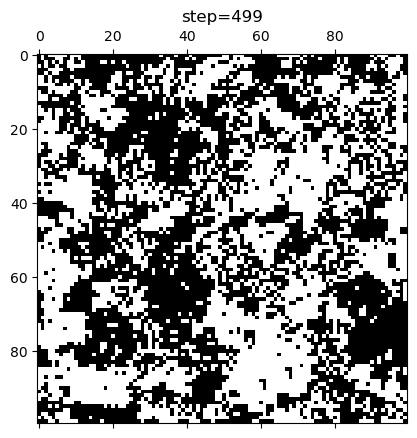
\includegraphics[width=0.3\textwidth]{img/fig3.png}
    \caption{临界温度 $T=T_c$ 时系统的位形}
    \label{fig3}
\end{figure}

\begin{figure}[htbp]
    \centering
    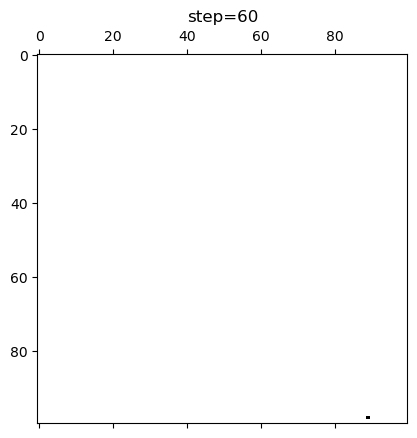
\includegraphics[width=0.3\textwidth]{img/fig4.png}
    \caption{低温 $T=1$ 时系统的位形,低温时系统发生自发磁化}
    \label{fig4}
\end{figure}

\begin{figure}[H]
    \centering
    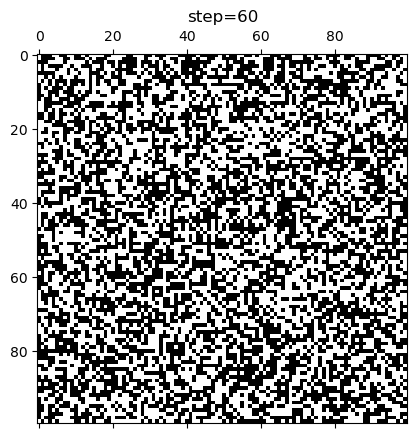
\includegraphics[width=0.3\textwidth]{img/fig5.png}
    \caption{高温 $T=10$ 时系统的位形,高温时系统宏观上不表现磁性}
    \label{fig5}
\end{figure}

\begin{figure}[H]
    \centering
    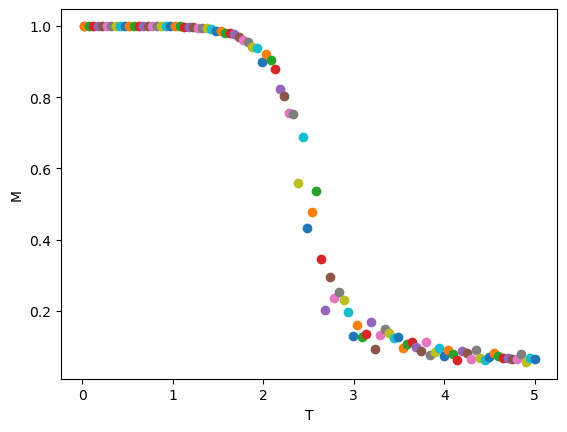
\includegraphics[width=0.3\textwidth]{img/fig6.png}
    \caption{平均磁矩随温度变化关系(取 $k=J=1$)理论给出在 $T_c=2/\ln(1+\sqrt{2})\approx 2.269 $ 处 发生相变}
    \label{fig6}
\end{figure}

\section{V. 结论}

本文通过介绍了数值模拟 Ising 模型的两种 Monte-Carlo 方法 : Single-spin-flip Dynamics 方法和Cluster-flip Dynamics 方法。通过这两种方法给出了各种热力学量随温度的变化关系,低温、临界温度、高温时系统的位形图。数值模拟结果与理论结果符合得很好。

% If in two-column mode, this environment will change to single-column
% format so that long equations can be displayed. Use
% sparingly.
%\begin{widetext}
% put long equation here
%\end{widetext}

% figures should be put into the text as floats.
% Use the graphics or graphicx packages (distributed with LaTeX2e)
% and the \includegraphics macro defined in those packages.
% See the LaTeX Graphics Companion by Michel Goosens, Sebastian Rahtz,
% and Frank Mittelbach for instance.
%
% Here is an example of the general form of a figure:
% Fill in the caption in the braces of the \caption{} command. Put the label
% that you will use with \ref{} command in the braces of the \label{} command.
% Use the figure* environment if the figure should span across the
% entire page. There is no need to do explicit centering.

% \begin{figure}
% \includegraphics{}%
% \caption{\label{}}
% \end{figure}

% Surround figure environment with turnpage environment for landscape
% figure
% \begin{turnpage}
% \begin{figure}
% \includegraphics{}%
% \caption{\label{}}
% \end{figure}
% \end{turnpage}

% tables should appear as floats within the text
%
% Here is an example of the general form of a table:
% Fill in the caption in the braces of the \caption{} command. Put the label
% that you will use with \ref{} command in the braces of the \label{} command.
% Insert the column specifiers (l, r, c, d, etc.) in the empty braces of the
% \begin{tabular}{} command.
% The ruledtabular enviroment adds doubled rules to table and sets a
% reasonable default table settings.
% Use the table* environment to get a full-width table in two-column
% Add \usepackage{longtable} and the longtable (or longtable*}
% environment for nicely formatted long tables. Or use the the [H]
% placement option to break a long table (with less control than 
% in longtable).
% \begin{table}%[H] add [H] placement to break table across pages
% \caption{\label{}}
% \begin{ruledtabular}
% \begin{tabular}{}
% Lines of table here ending with \\
% \end{tabular}
% \end{ruledtabular}
% \end{table}

% Surround table environment with turnpage environment for landscape
% table
% \begin{turnpage}
% \begin{table}
% \caption{\label{}}
% \begin{ruledtabular}
% \begin{tabular}{}
% \end{tabular}
% \end{ruledtabular}
% \end{table}
% \end{turnpage}

% Specify following sections are appendices. Use \appendix* if there
% only one appendix.
%\appendix
%\section{}

% If you have acknowledgments, this puts in the proper section head.
%\begin{acknowledgments}
% put your acknowledgments here.
%\end{acknowledgments}

% Create the reference section using BibTeX:

\section*{References}
\begin{thebibliography}{99}
    
    \bibitem{01} Ivaneyko, Dmytro, et al. "Criticality of the random-site Ising model: Metropolis, Swendsen-Wang and Wolff Monte Carlo algorithms." arXiv preprint cond-mat/0501291 (2005).

    \bibitem{02} Onsager, Lars. "Crystal statistics. I. A two-dimensional model with an order-disorder transition." Physical Review 65.3-4 (1944): 117.

    \bibitem{03} Ernst, Ising. "Beitrag zur theorie des ferromagnetismus." Zeitschrift für Physik A Hadrons and Nuclei 31.1 (1925): 253-258.

\end{thebibliography}

\end{document}
%
% ****** End of file apstemplate.tex ******

